\documentclass{article}

\usepackage[a4paper, left=.5in, right=.5in, top=.25in, bottom=0.5in]{geometry}
\usepackage{tikz}
\usepackage{multicol}
\usepackage{mathtools}
\usepackage{booktabs}
\usepackage{tabularx}

\title{LiDAR Portfolio\\\large Software Product Engineering}
\author{Daniel Jones (ae18592), Jed Priest, Jarrod Doyle, Alex Asher}
\date{}

\begin{document}
\maketitle
\begin{multicols}{2}
    \section{Introduction}
    Lloyds Registrar has requested a web-based solution to visualize and compute various statistics between two sets of data: LiDAR and the existing trusted fixed measurement device. This is to build confidence that the LiDAR system is fully functional and giving accurate readouts before being deployed to any potential windfarm location.
\par Before the LiDAR system can be deemed accurate it must pass all KPIs (key performance indicators). Each of the KPIs will be displayed in the web application in relevant charts to show whether the KPI has been met. Each of the KPIs will be implemented in different releases with the ones giving the most information of the technical performance implemented first.
\par The team envisions the product to have two views: a simplified investor view and a technical view both of which display the data in a clean concise way appropriate for the respective viewer. An inaugural mockup that represents our vision for the GUI on our platform can be seen below:
    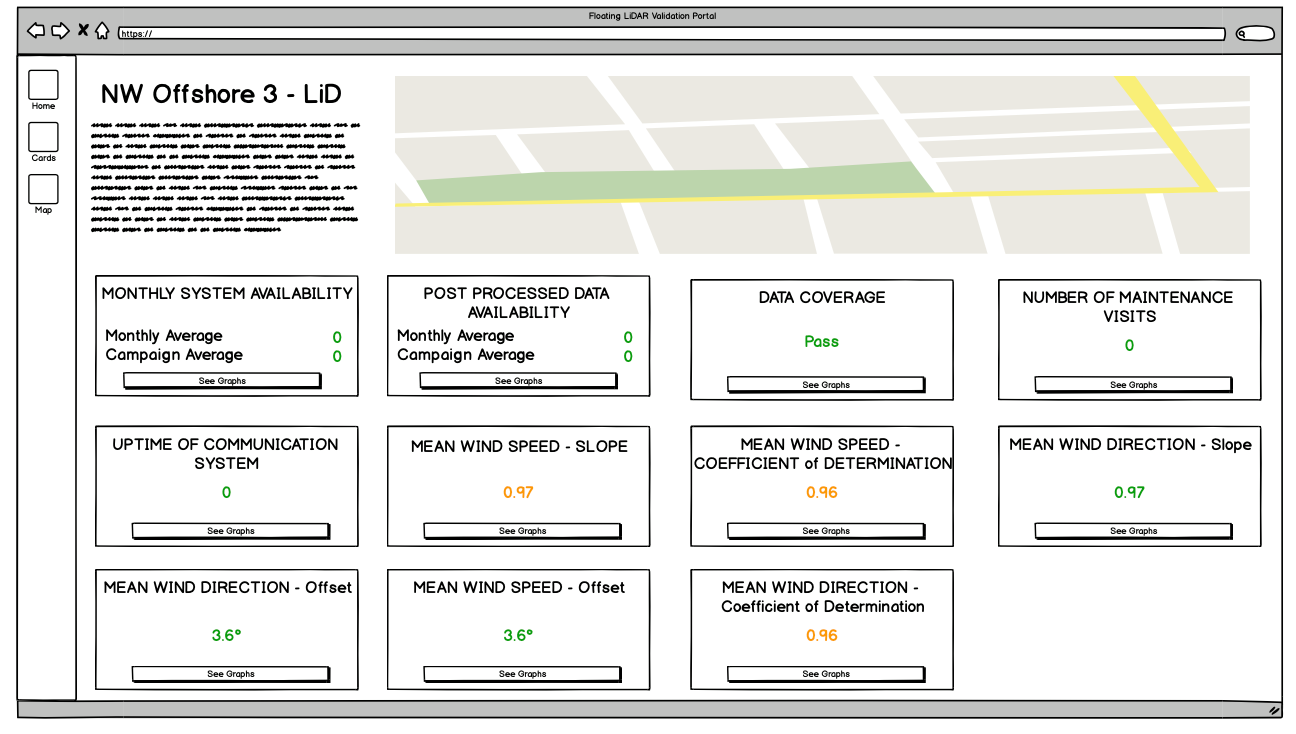
\includegraphics[width=\linewidth]{mock1.png}
    
    \section{Requirements}
    The requirements set out below describe the key features that are required to make the platform successful for the client. Functional requirements denote features that are essential to the platform's success and non-functional requirements refer to those that aid and improve the platforms effectiveness.
    \subsection{Functional requirements}
    \begin{itemize}
        \item Data must be displayed in the web browser 
        \item Calculate all Key Performance Indicators to be calculated correctly 
        \item Investor view and a technical view. 
        \item Can select specific Lidar device to look at. 
        \item Investor View: 
        \begin{itemize}
            \item A dumbed down version but can still click to see technical view. 
            \item “Make the reader feel like they’re smart when they don’t know the intricate details” 
        \end{itemize}
        \item Technical view: 
            \begin{itemize}
                \item Technical view to see if devices are working. 
                \item Detailed stats 
            \end{itemize}
    \end{itemize}
    \subsection{Non-functional requirements}
    \begin{itemize}
        \item Data must be processed faster than the manual excel method 
        \item Data must be presented in a clear format like the technical documents 
        \item Must have a friendly and easy to use interface  
    \end{itemize}
    \subsection{Future Ambitions Requirements}
    \begin{itemize}
        \item To be able to predict a completion date by using weather predictions.
    \end{itemize}
    \subsection{KPIs (in order)}
    \begin{tabularx}{\linewidth}{XXX}
        Indicator & Acceptance Criteria (\%) & Client Comments \\
        \toprule
        Monthly System Availability - 1 month average & $\geq 90$ & Ignore - easy to add later but will be 100\% for sample data \\
        Overall system availability - campaign average & $\geq 95$ & Ignore - easy to add later but will be 100\% for sample data \\
        Monthly post processed data availability - 1 month average & $\geq 80$ & Ca wait for second release \\
        Overall post processed data availability & $ \geq 85$ & Ignore - easy to add later buy 100\% for data sample \\
        Data coverage & 
        \begin{enumerate}
            \item Minimum of 40 data points in each $1ms^{-1}$ wide reference wind speed bin centred between $2.5ms^{-1}$ and $11.5ms^{-1}$ i.e. covering a range between 2 and $12ms^{-1}$
            \item Minimum of 40 data points required in each $2ms^{-1}$ wide reference wind speed bin centred on $13ms^{-1}$ and $15ms^{-1}$ i.e. covering a range between 12 and $16ms^{-1}$
        \end{enumerate}
    \end{tabularx}
    \vfill\null\columnbreak{}
    \vfill\null{}
\end{multicols}
\end{document}
